\section{评估审计与分层结果}
\label{app:evalaudit}
\subsection{有效试验与标签修正}
最终数据由五种方法各96次有效记录构成，覆盖四类物体、12个位置和每条件两次重复。
segNoQtoken在方块$(1,0)$的一次测试中，自动评估器判为成功，操作者确认目标停在区域边缘并保存为失败；本文按保存标签统计。
该组在纸球$(3,0)$的一次18.7 s手动中止被确认为无效，已排除，并由一条正常执行至40 s、结果为失败的补采记录替换。
补采后没有缺失或重复的物体--位置--重复编号组合，全部480条记录均正常退出且没有手动中止标记。
原有ACT、DP、RGBQtoken和viewQtoken四组记录保持不变。

\subsection{统计口径}
跨方法比较在物体--位置区组内进行。
每个区组的两方法共四个二值结果，在固定总成功数下按每方法两次重新分配；
将48个区组的超几何分布卷积，得到总体成功次数差的精确零假设分布。
分物体分析只使用对应的12个区组，四类物体全部40项方法比较构成统一校正族。

关联检验以各分组汇总成功次数的平方和为离散度统计量。
位置检验在物体内置换结果，物体检验在位置内置换，
列检验在物体--行内置换，行检验在物体--列内置换。
使用200000次Monte Carlo置换及加一修正，最小可报告未校正$p$值约为$5\times10^{-6}$，不将其写为零。
总体方法差异与关联检验分别使用独立的10项和20项Holm校正族。
比例区间为总体二值计数的Wilson描述性区间，并未建模跨训练种子波动或逐条件的不同成功概率。

\subsection{完整物体--位置矩阵}
图~\ref{fig:objectpositions}呈现全部240个方法--物体--位置单元，每格两次。
同一列比较固定物体在不同位置的表现，同一行跨列比较同一方法的不同物体；
相同网格坐标则用于比较不同物体在同一位置的结果。
\begin{figure*}[p]
\centering
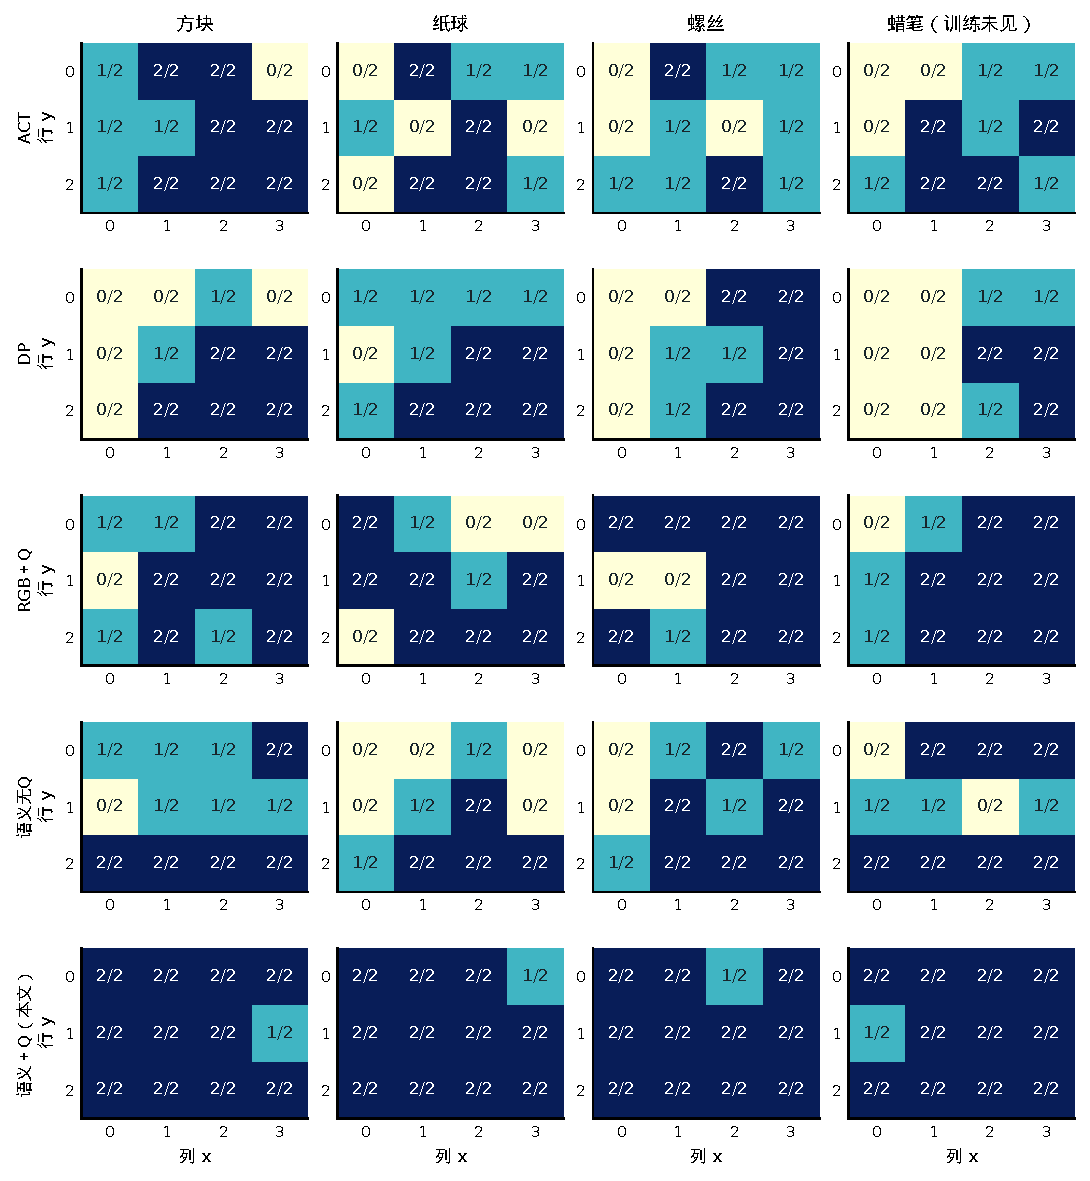
\includegraphics[width=0.94\textwidth,height=0.80\textheight,keepaspectratio]{figures/results_20261023/object_position_zh.pdf}
\caption{完整的物体--位置结果。每个小面板为四列三行测试网格，每格标注成功次数/2，所有面板统一色阶：浅色0/2，中间色1/2，深色2/2。行对应方法，列对应物体；蜡笔为训练未见类别。}
\label{fig:objectpositions}
\end{figure*}
